\section{Results}\label{sec:results}

The absolute mean error by coordination mechanism per voting mechanism is graphed in
\autoref{fig:vm-col-cm-hue-error-as-percent-of-space-abs-mean}.
There are a few trends that are immediately identifiable.
First, error unsurprisingly increases as the number of inactive agents increases.
This is true with two notable exceptions: first, the Active Only/Median
mechanism combination has a somewhat sawtooth shape.
This is due to the Median mechanisms always choosing a specific agent's preference
instead of aggregating to some more preferential in-between value.

The second exception is that Mean mechanism consistently dips when all but one agent
become delegators.
This is because we take the mean of the constituents and the proxy, then apply the
voting mechanism on the set of proxy-constituent votes.
Since there is only one proxy-constituent vote, the result is the vote itself.
Essentially, the coordination mechanism replaces the voting mechanism.

We can also see the Mean and Median coordination mechanisms generally yield similar
amounts of error.
In particular, when either of these mechanisms is combined with the Mean voting
mechanism the results are very similar to when all agents are active and able to vote.

Notably, the Expert coordination mechanism works worse than the others as the number
of delegators reaches a significant portion of the population.
In particular, the Expert mechanism tracks nearly identically to Active Only when
using the Midrange voting mechanism.
Depending on the use case, this may or may not be beneficial.
If we are attempting to find the best result for all agents, this mechanism may yield
undesirable results.
However, if we are attempting to exploit the experts experience, as described
by~\cite{Miller1969}, this error could actually be considered the improvement over
the original result.
This is because the experts were able to influence and change the vote, presumably
bringing it closer to what their expertise dictates.
Nevertheless, when the number of delegators is low, the Expert mechanism works
similarly to the other coordination mechanisms.

Importantly, it is clear that using proxy voting, regardless of the mechanisms used,
is better than losing information by not allowing inactive agents to vote in any way.

\begin{landscape}
    \begin{figure}[p]
        \centering
        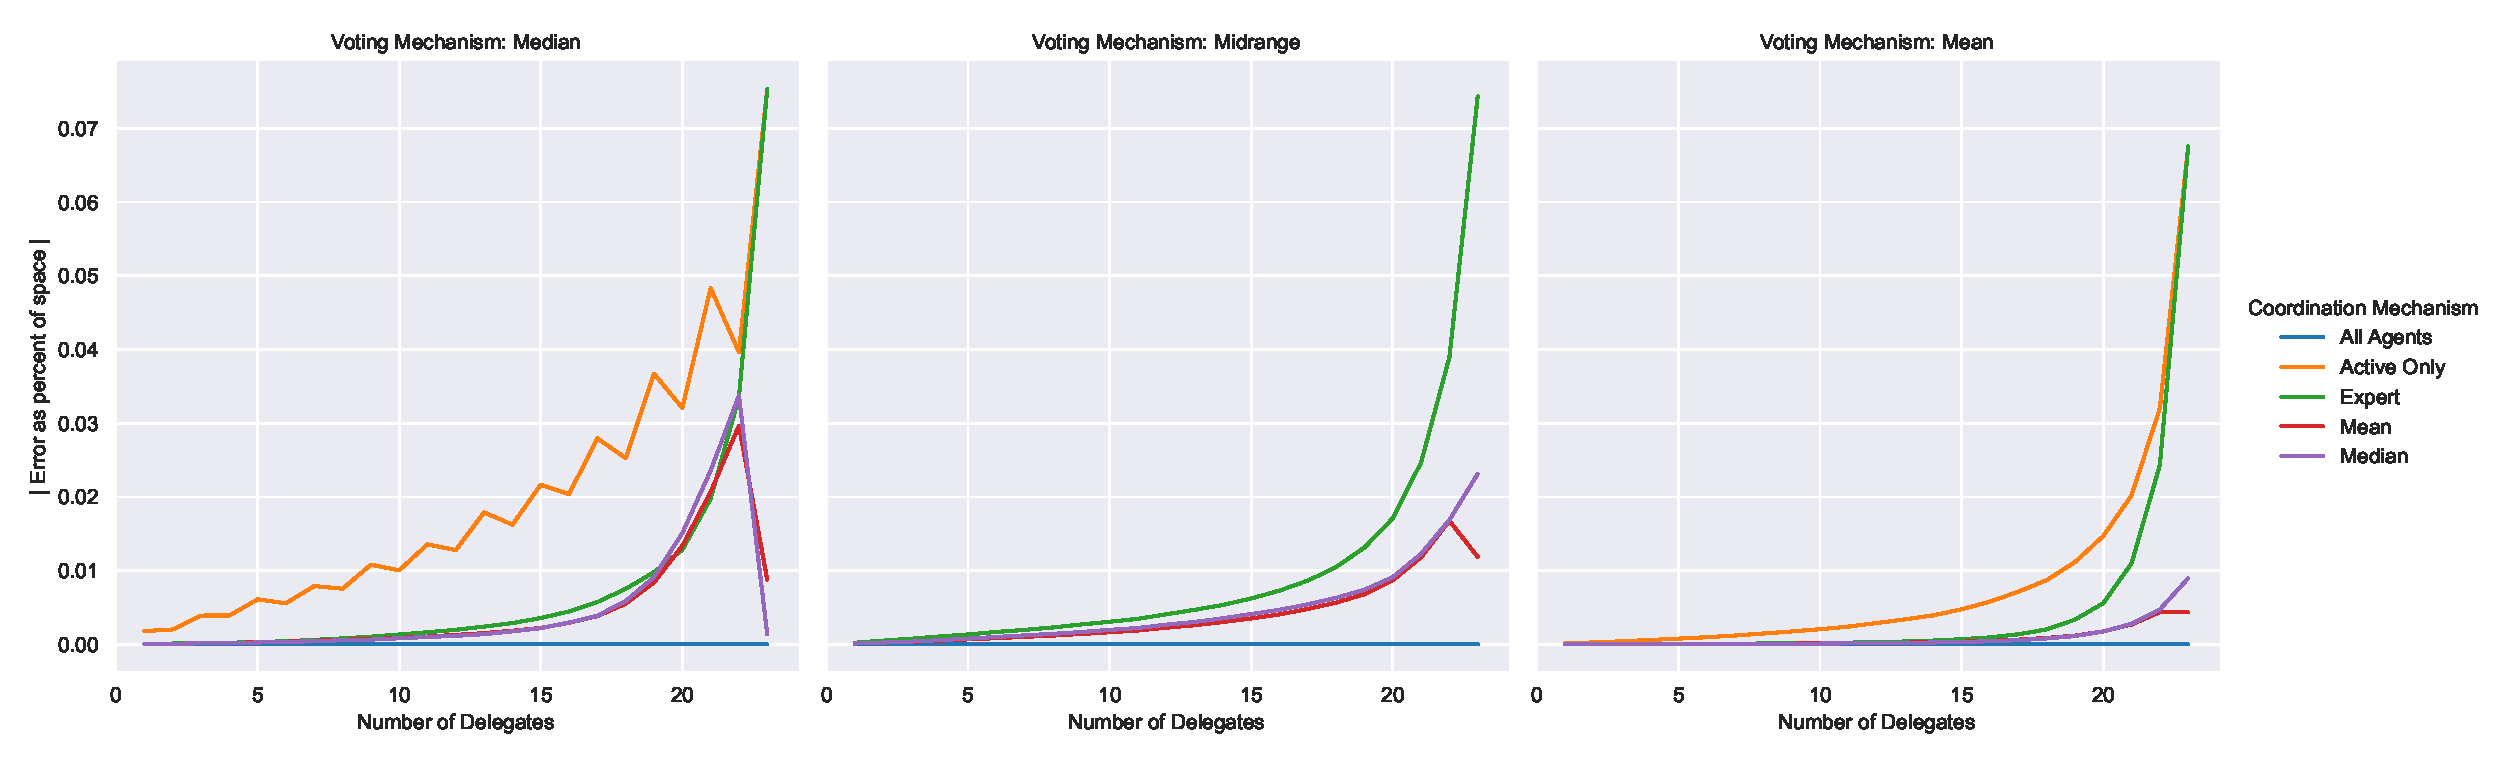
\includegraphics[scale=0.55]
        {content/chapter2/figures/vm_col_cm_hue_error_as_percent_of_space_abs_mean}
        \caption{
            The absolute mean error by coordination mechanism per voting mechanism.
            Note All Agents represents when all agents are voting, meaning no proxy
            voting is used and all agents are present.
            Similarly, Active Only represents when proxy voting is not used and not
            all agents are present, and when proxies lose their constituents.
        }
        \label{fig:vm-col-cm-hue-error-as-percent-of-space-abs-mean}
    \end{figure}
\end{landscape}

% \section{Conclusions}\label{sec:conclusions}?
% \section{Future Work}\label{sec:future-work}?
